\documentclass[a4paper,11pt,openright]{report}
\setlength{\parindent}{0pt} % set noindent for entire file

\usepackage[utf8]{inputenc}
\usepackage[a4paper, top=2cm, left=1cm, right=1.5cm]{geometry}
\usepackage{xcolor,graphicx}
\usepackage{amsmath}
\usepackage{setspace}
\usepackage{sectsty}
\usepackage{etoolbox}
\usepackage{enumitem}
\usepackage{listings}
\usepackage{times}

\graphicspath{ {/home/saran/Analytics/May_04/} }

\lstdefinestyle{mystyle}{
	backgroundcolor=\color{white},
	basicstyle=\ttfamily\footnotesize,
	breakatwhitespace=false,
	breaklines=true,
	captionpos=b,
	keepspaces=true,
	showspaces=false,
	showstringspaces=false,
	showtabs=false,
	tabsize=4
}

\lstset{style=mystyle}

\begin{document}
\singlespacing
\pagestyle{plain}

\begin{center}
\textbf{Assignment Binomial Distribution} \\
Date: 04/05/2020 \hspace{2mm} Name: D.Saravanan
\end{center}

\vspace{10px}

\begin{enumerate}

\item[1.] For a Binomial Distribution parameter $n = 5$ and $p = 0.3$ Find the probabilities
of getting

\begin{enumerate}

\item[a)] At least $3$ successes \\
The probability that a random variable $X$  with binomial distribution $B(n,p)$ is equal to
the value $k$, where $k = 0, 1,...n$, is given by

\begin{equation*}
P(X = k) = \binom nk p^{k} (1-p)^{n-k} = \frac{n!}{k! (n-k)!} p^{k} (1-p)^{n-k}
\end{equation*}

\begin{equation*}
\begin{split}
		P(X \geq 3) & = P(X = 3) + P(X = 4) + P(X = 5) \\ 
		& = \binom 53 (0.3)^{3} (1-0.3)^{2} + \binom 54 (0.3)^{4} (1-0.3) + \binom 55 (0.3)^{5} \\ 
		& = \frac{5!}{3! (5-3)!} (0.3)^{3} (0.7)^{2} + \frac{5!}{4! (5-4)!} (0.3)^{4} (0.7) + \frac{5!}{5! (5-5)!} (0.3)^{5} \\
		& = 0.1323 + 0.0283 + 0.0024 \\
		& = 0.1630
\end{split}
\end{equation*}

\item[b)] At most $3$ successes \\ \\
Method 1:
\begin{equation*}
\begin{split}
		P(X \leq 3) & = P(X = 0) + P(X = 1) + P(X = 2) + P(X = 3) \\ 
		& = \binom 50 (1-0.3)^{5} + \binom 51 (0.3) (1-0.3)^{4} + \binom 52 (0.3)^{2} (1-0.3)^{3} + \binom 53 (0.3)^{3} (1-0.3)^{2} \\
		& = \frac{5!}{0! (5-0)!} (0.7)^{5} + \frac{5!}{1! (5-1)!} (0.3) (0.7)^{4} + \frac{5!}{2! (5-2)!} (0.3)^{2} (0.7)^{3} + \frac{5!}{3! (5-3)!} (0.3)^{3} (0.7)^{2} \\
		& = 0.1681 + 0.3601 + 0.3087 + 0.1323 \\
		& = 0.9692
\end{split}
\end{equation*}

Method 2:
\begin{equation*}
\begin{split}
		P(X \leq 3) & = 1 - P(X > 3) \\
		& = 1 - (P(X = 4) + P(X = 5)) \\
		& = 1 - \left( \binom 54 (0.3)^{4} (1-0.3) + \binom 55 (0.3)^{5} \right) \\
		& = 1 - \left( \frac{5!}{4! (5-4)!} (0.3)^{4} (0.7) + \frac{5!}{5! (5-5)!} (0.3)^{5} \right) \\
		& = 1 - (0.0283 + 0.0024) \\
		& = 0.9692
\end{split}
\end{equation*}

\pagebreak

\item[c)] Exactly $3$ failures \\
\begin{equation*}
\begin{split}
		P(X = 2) & = \binom 52 (0.3)^{2} (1-0.3)^{3} \\
		& = \frac{5!}{2! (5-2)!} (0.3)^{2} (0.7)^{3} \\
		& = 0.3087
\end{split}
\end{equation*}

\end{enumerate}

Program:
\lstinputlisting[language=Python]{bdist.py}

\pagebreak

Output:
\lstinputlisting{outputb1.txt}

\vspace{1cm}

Program: Binomial Distribution using Scipy package
\lstinputlisting[language=Python]{bdistribution.py}

Output:
\lstinputlisting{outputb2.txt}

\item[2.] If on an average one vessel in every ten is wrecked, find the probability that out
of five vessels expected to arrive, four at least will arrive safely. \\

The probability of success, $p = 0.9$ and the number of observations, $n = 5$.

\begin{equation*}
\begin{split}
		P(X \geq 4) & = P(X = 4) + P(X = 5) \\
		& = \binom 54 (0.9)^{4} (1-0.9) + \binom 55 (0.9)^{5} \\
		& = \frac{5!}{4! (5-4)!} (0.9)^{4} (0.1) + \frac{5!}{5! (5-5)!} (0.9)^{5} \\
		& = 0.3280 + 0.5905 \\
		& = 0.9185
\end{split}
\end{equation*}

Program: 
\lstinputlisting[language=Python]{vessels.py}

Output:
\lstinputlisting{outputb3.txt}

\item[3.] Five coins are tossed 3,200 times.

Program:
\lstinputlisting[language=Python]{binormdist.py} \begin{enumerate}

\pagebreak

\item[a)] Find the Frequencies of the distribution of heads and tabulate the results.

\lstinputlisting{outputb4.txt}

%figure_1
\begin{figure}[ht!]
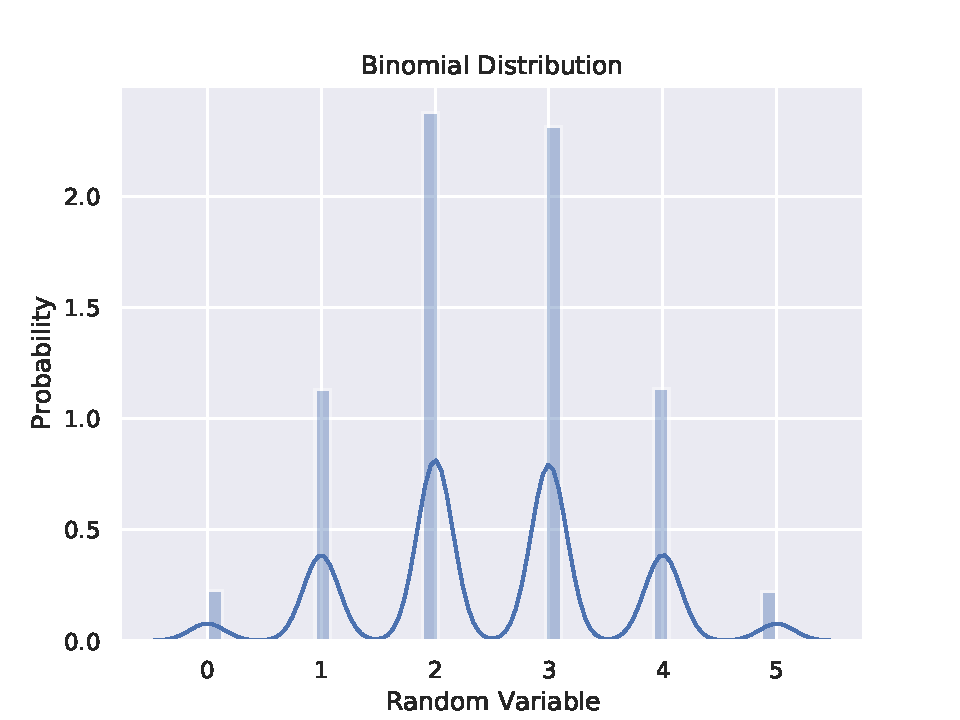
\includegraphics[width=18cm,height=9cm,keepaspectratio]{binormdistplot.pdf}
\centering
\end{figure}

\vspace{2cm}

\item[b)] Calculate the mean number of sucess and standard deviation.
		\begin{enumerate}
				\item[ ] Mean, $\mu_{X} = np = 5 \times 0.5 = 2.5$
				\item[ ] Variance, $\sigma^{2}_{X} = np(1-p) = 5 \times 0.5 \times (1-0.5) = 1.25$
				\item[ ] Standard Deviation, $\sigma_{X} = \sqrt{np(1-p)} = \sqrt{1.25} = 1.12$
		\end{enumerate}

Output:
\lstinputlisting{outputb5.txt}


\end{enumerate}

\end{enumerate}
\end{document}
